\documentclass{article}
\usepackage[english,russian]{babel}
\usepackage{textcomp}
\usepackage{geometry}
  \geometry{left=2cm}
  \geometry{right=1.5cm}
  \geometry{top=1.5cm}
  \geometry{bottom=2cm}
\usepackage{tikz}
\usepackage{multicol}
\usepackage{listings}
\pagenumbering{gobble}

\lstdefinestyle{csMiptCppStyle}{
  language=C++,
  basicstyle=\linespread{1.1}\ttfamily,
  columns=fixed,
  fontadjust=true,
  basewidth=0.5em,
  keywordstyle=\color{blue}\bfseries,
  commentstyle=\color{gray},
  texcl=true,
  stringstyle=\ttfamily\color{orange!50!black},
  showstringspaces=false,
  %numbers=false,
  numbersep=5pt,
  numberstyle=\tiny\color{black},
  numberfirstline=true,
  stepnumber=1,      
  numbersep=10pt,
  backgroundcolor=\color{white},
  showstringspaces=false,
  captionpos=b,
  breaklines=true
  breakatwhitespace=true,
  xleftmargin=.2in,
  extendedchars=\true,
  keepspaces = true,
  tabsize=4,
  upquote=true,
  emph = {override, final},
  emphstyle={\color{blue}\bfseries},
}
\lstdefinestyle{csMiptCppBorderStyle}{
  style=csMiptCppStyle,
  framexleftmargin=5mm, 
  frame=shadowbox, 
  rulesepcolor=\color{gray}
}

\lstset{style=csMiptCppStyle}
\lstset{literate={~}{{\raisebox{0.5ex}{\texttildelow}}}{1}}


\begin{document}
\title{Семинар \#3: Динамический полиморфизм \vspace{-5ex}}\date{}\maketitle

\section*{Полиморфизм}
\textbf{Полиморфизм} -- это способность функций обрабатывать данные разных типов.

Полиморфизм существует в большинстве языков программирования в том или ином виде. Например, рассмотрим следующую программу на языке Python:
\begin{lstlisting}[language=Python]
def plus(a, b):
    return (a + b)

print(plus(10, 20))        # Напечатает 30
print(plus("Cat", "Dog"))  # Напечатает CatDog
\end{lstlisting}
Здесь функция \texttt{plus} является полиморфной, так как может работать с данными разных типов.

\subsection*{Статический полиморфизм}
Полиморфизм в языке C++ мы уже частично прошли. Ведь такие возможности языка как перегрузка функций и шаблоны позволяют писать функции, которые работают с разными типами:
\begin{lstlisting}[style=csMiptCppStyle]
#include <iostream>
#include <string>
using namespace std::string_literals;

template<typename T>
T plus(T x, T y)
{
	return x + y;
}

int main()
{
	std::cout << plus(10, 20) << std::endl;          // Напечатает 30
	std::cout << plus("Cat"s, "Dog"s) << std::endl;  // Напечатает CatDog
}
\end{lstlisting}
Однако, в этом случае то, какая функция будет вызвана, определяется на этапе компиляции: при раскрытии шаблона или при выборе перегрузки. Вид полиморфизма, при котором вызываемая функция определяется на этапе компиляции, называется статическим полиморфизмом. 
\subsection*{Динамический полиморфизм}
Вид полиморфизма, при котором вызываемая функция определяется на этапе выполнения, называется динамическим полиморфизмом. При динамическом полиморфизме даже неизвестен тип аргумента, приходящего на вход функции на этапе компиляции, он становится известен только на этапе выполнения. Таким образом в языке должны существовать объекты, которые могут "менять"{} свой тип.\\
В языке Python динамический полиморфизм просто встроен в язык и любые объекты могут менять свой тип:
\begin{lstlisting}[language=Python]
a, b = 10, 20
print(plus(a, b))     # Напечатает 30, тип объектов a и b - int
a, b = "Cat", "Dog"
print(plus(a, b))     # Напечатает CatDog, тип объектов a и b - строка
\end{lstlisting}
В языке С++ у всех объектов фиксированный тип, а динамический полиморфизм достигается с помощью наследования и механизма виртуальных функций.

\newpage
\section*{Виртуальные функции}
Виртуальные функции (также известные как виртуальные методы) -- это механизм, который позволяет осуществлять динамический полиморфизм в языке C++.
Виртуальные функции позволяют динамически определять, какая функция будет вызвана в зависимости от типа объекта, а не типа указателя или ссылки, указывающего на этот объект.
Виртуальные функции не следует путать с виртуальным наследованием, это разные вещи.

Чтобы указать, что какой-либо метод является виртуальным, нужно использовать ключевое слово \texttt{virtual} в объявлении метода в базовом классе. После этого этот метод, а также все методы с такой же сигнатурой во всех производных классах станут виртуальными. Использовать \texttt{virtual} в объявлениях методов производных классов необязательно. Виртуальный метод отличается от обычного следующим:

\begin{center}
\textit{Если в программе возникнет ситуация когда указатель (или ссылка) на базовый класс будет указывать на объект производного класса, то при вызове виртуального метода через этот указатель (или ссылку) будет вызываться метод производного класса, а не метод базового класса.}
\end{center}

Рассмотрим пример класса \texttt{Bob}, который наследуется от класса \texttt{Alice} и у этих классов есть виртуальные методы под названием \texttt{say}. Метод \texttt{say} в классе \texttt{Alice} стал виртуальным, так как мы пометили его ключевым словом \texttt{virtual}. Метод \texttt{say} в классе \texttt{Bob} также будет виртуальным, потому что он переопределяет виртуальный метод в родительском классе. Таким образом, независимо от того пометим мы метод \texttt{Bob::say} словом \texttt{virtual} или нет, он будет виртуальным.


\begin{lstlisting}[style=csMiptCppBorderStyle]
struct Alice 
{
    virtual void say() 
    {
    	std::cout << "Alice" << std::endl;
    }
};

struct Bob : public Alice 
{
    void say() 
    {
    	std::cout << "Bob" << std::endl;
    }
};
\end{lstlisting}
Виртуальные методы отличаются от обычных методов тем, что если мы вызываем этот метод через указатель (или ссылку) на объект, то будет вызываться метод класса объекта на который указывает этот указатель.
\begin{lstlisting}[style=csMiptCppBorderStyle]
Bob b;
Alice* pa = &b;
pa->say();  // Вызовется метод Bob::say, так как pa указывает на объект типа Bob
            // Если бы метод say не был бы виртуальным, то вызвался бы метод Alice::say,
            // так как указатель имеет тип Alice*
\end{lstlisting}



Обратите внимание, что виртуальные функции работают в случае когда есть указатель (или ссылка) на базовый класс, который указывает на объект производного класса, но не работают когда, например, объект базового класса инициализирован объектом производного класса.

\newpage
\subsection*{Объект базового класса, инициализированный объектом производного}
\begin{multicols}{2} \noindent
\begin{lstlisting}[style=csMiptCppBorderStyle]
#include <iostream>
struct Alice 
{
    void say() 
    {
    	std::cout << "Alice" << std::endl;
    }
};
struct Bob : public Alice 
{
    void say() 
    {
    	std::cout << "Bob" << std::endl;
    }
};

int main() 
{
    Bob b;
	Alice a = b;
    a.say();  // Напечатает Alice
}
\end{lstlisting}


\begin{lstlisting}[style=csMiptCppBorderStyle]
#include <iostream>
struct Alice 
{
    virtual void say() 
    {
    	std::cout << "Alice" << std::endl;
    }
};
struct Bob : public Alice 
{
    void say() 
    {
    	std::cout << "Bob" << std::endl;
    }
};

int main() 
{
    Bob b;
	Alice a = b;
    a.say();  // Всё равно напечатает Alice
}
\end{lstlisting}
\end{multicols}

\subsection*{Указатели на базовый класс, хранящие адрес объекта производного класса}
\begin{multicols}{2}\noindent
\begin{lstlisting}[style=csMiptCppBorderStyle]
#include <iostream>
struct Alice 
{
    void say() 
    {
    	std::cout << "Alice" << std::endl;
    }
};
struct Bob : public Alice 
{
    void say() 
    {
    	std::cout << "Bob" << std::endl;
    }
};

int main() 
{
    Bob b;
	Alice* pa = &b;
    pa->say();  // Напечатает Alice
}
\end{lstlisting}


\begin{lstlisting}[style=csMiptCppBorderStyle]
#include <iostream>
struct Alice 
{
    virtual void say() 
    {
    	std::cout << "Alice" << std::endl;
    }
};
struct Bob : public Alice 
{
    void say() 
    {
    	std::cout << "Bob" << std::endl;
    }
};

int main() 
{
    Bob b;
	Alice* pa = &b;
    pa->say();  // Напечатает Bob
}
\end{lstlisting}
\end{multicols}

\newpage
\subsection*{Вызов виртуальных функций из методов класса}
Ещё один случай когда работают виртуальные функции -- если мы вызываем виртуальный метод из другого метода (не важно виртуального или не виртуального).

\begin{multicols}{2}\noindent
\begin{lstlisting}[style=csMiptCppBorderStyle]
#include <iostream>
struct Alice 
{
    void say() 
    {
    	std::cout << "Alice" << std::endl;
    }    
    
    void func() 
    {
    	say();
    }
};

struct Bob : public Alice 
{
    void say() 
    {
    	std::cout << "Bob" << std::endl;
    }
};

int main() 
{
    Bob b;
	b.func();  // Напечатает Alice
}
\end{lstlisting}


\begin{lstlisting}[style=csMiptCppBorderStyle]
#include <iostream>
struct Alice 
{
    virtual void say() 
    {
    	std::cout << "Alice" << std::endl;
    }    
    
    void func() 
    {
    	say();
    }
};

struct Bob : public Alice 
{
    void say() 
    {
    	std::cout << "Bob" << std::endl;
    }
};

int main() 
{
    Bob b;
	b.func();  // Напечатает Bob
}
\end{lstlisting}
\end{multicols}


\subsection*{Как виртуальные функции приводят к динамическому полиморфизму}
Указатель типа \texttt{Alice*} может указывать как на объект типа \texttt{Alice} или на объект типа \texttt{Bob} (или на объект любого другого наследника \texttt{Alice}). В зависимости от того куда указывает этот указатель будет вызываться та или иная виртуальная функция. То, на какой объект будет указывать \texttt{Alice}, часто будет известно только на этапе выполнения.
Таким образом метод \texttt{say} может работать либо с объектом типа \texttt{Alice} либо с объектом типа \texttt{Bob} и то, с каким объектом будет работать данный метод, зависит от значения указателя \texttt{Alice*} и будет известно только на стадии выполнения.
\begin{lstlisting}[style=csMiptCppBorderStyle]
Alice a; Bob b;

Alice* p;
int x;
std::cin >> x;
if (x == 0) p = &a;
else        p = &b;

p->say();  // Напечатает Alice или Bob, в зависимости от того, какое число было
           // введено на этапе выполнения
\end{lstlisting}

\newpage
\subsection*{Виртуальные функции в конструкторах и деструкторах}
Если производный класс вызывает конструктор базового класса (это происходит автоматически в перед вызовом конструктора производного класса) и в конструкторе базового класса вызывается виртуальный метод, то вызовется метод базового класса. То есть в этом случае виртуальность метода "не работает".
Это происходит просто потому что объект производного класса не может вызывать свои методы, так как он ещё не готов к этому. 
\begin{lstlisting}[style=csMiptCppBorderStyle]
#include <iostream>
struct Alice 
{
    Alice()     {say();}
    void func() {say();}
    virtual void say() 
    {
    	std::cout << "Alice" << std::endl;
    }
};

struct Bob : public Alice 
{
    void say() 
    {
    	std::cout << "Bob" << std::endl;
    }
};

int main() 
{
    Bob b;     // Вызовет конструктор Alice(), который вызовет Alice::func и напечатает Alice
    b.func();  // Вызовет Bob::func и напечатает Bob
}
\end{lstlisting}
Похожая ситуация будет и при вызове виртуального метода в деструкторе:
\begin{lstlisting}[style=csMiptCppBorderStyle]
#include <iostream>
struct Alice 
{
    virtual void say() {std::cout << "Alice" << std::endl;}
    void func() {say();}
    virtual ~Alice()    {say();}
};

struct Bob : public Alice 
{
    void say() {std::cout << "Bob" << std::endl;};
    ~Bob() {}
};

int main() 
{
    Bob b;
    b.func();  // Напечатает Bob
               // Напечатает Alice при уничтожении объекта
}
\end{lstlisting}



\subsection*{Виртуальный деструктор}
Одна из самых распространённых ошибок при работе с виртуальными функциями -- это забыть сделать деструктор базового класса виртуальным. Это может привести к тому, что при удалении объекта производного класса, через указатель на базовый класс, не будет вызываться деструктор производного класса. Это может привести к ошибкам, например в примере ниже это приводит к утечке памяти.

\begin{lstlisting}[style=csMiptCppBorderStyle]
#include <iostream>

struct Alice 
{
    virtual void say() 
    {
    	std::cout << "Alice" << std::endl;
    }
};

struct Bob : public Alice 
{
	char* data;
	
	Bob()
	{
		std::cout << "Allocating Memory" << std::endl;
		data = new char[100];		
	}
	
    void say() 
    {
    	std::cout << "Bob" << std::endl;
    }
    
    ~Bob()
    {
    	std::cout << "Freeing Memory" << std::endl;
    	delete[] data;
    }
};

int main() 
{
	Alice* p = new Bob;  // Напечатает Allocating Memory
    p->say();            // Напечатает Bob, так как функция say - виртуальная
    delete p;            // НЕ напечатает Freeing Memory, так как деструктор НЕ виртуальный
}
\end{lstlisting}

Решение проблемы -- нужно просто пометить деструктор базового класса словом \texttt{virtual}, то есть добавить в класс \texttt{Alice} строку:
\begin{lstlisting}[style=csMiptCppStyle]
virtual ~Alice() {}
\end{lstlisting}

\subsection*{\texttt{override} и \texttt{final}}

\subsection*{Полиморфизм и умные указатели}

\subsection*{Как программа понимает, какой виртуальный метод вызывать}
Размер объектов полиморфных типов. Скрытый указатель на таблицу виртуальных функций.




\newpage
\section*{Реализация механизма виртуальных функций}
\noindent\begin{minipage}{.43\textwidth}
\begin{lstlisting}[style=csMiptCppStyle]
#include <iostream>
struct Alice 
{
	int x;
    virtual void say() 
    {
    	std::cout << "Alice Say\n";
    }
    virtual void walk() 
    {
    	std::cout << "Alice Walk\n";
    }
};

struct Bob : public Alice 
{
	int y;
    virtual void say() 
    {
    	std::cout << "Bob Say\n";
    }
    virtual void walk() 
    {
    	std::cout << "Bob Walk\n";
    }
};

int main() 
{
    Alice a {10};
    Bob b {20, 30};
    
    Alice* p = &a;
    p->say();  // Напечатает Alice Say
    
    p = &b;
    p->say();  // Напечатает Bob Say
}
\end{lstlisting}
\end{minipage}
\begin{minipage}{.5\textwidth}
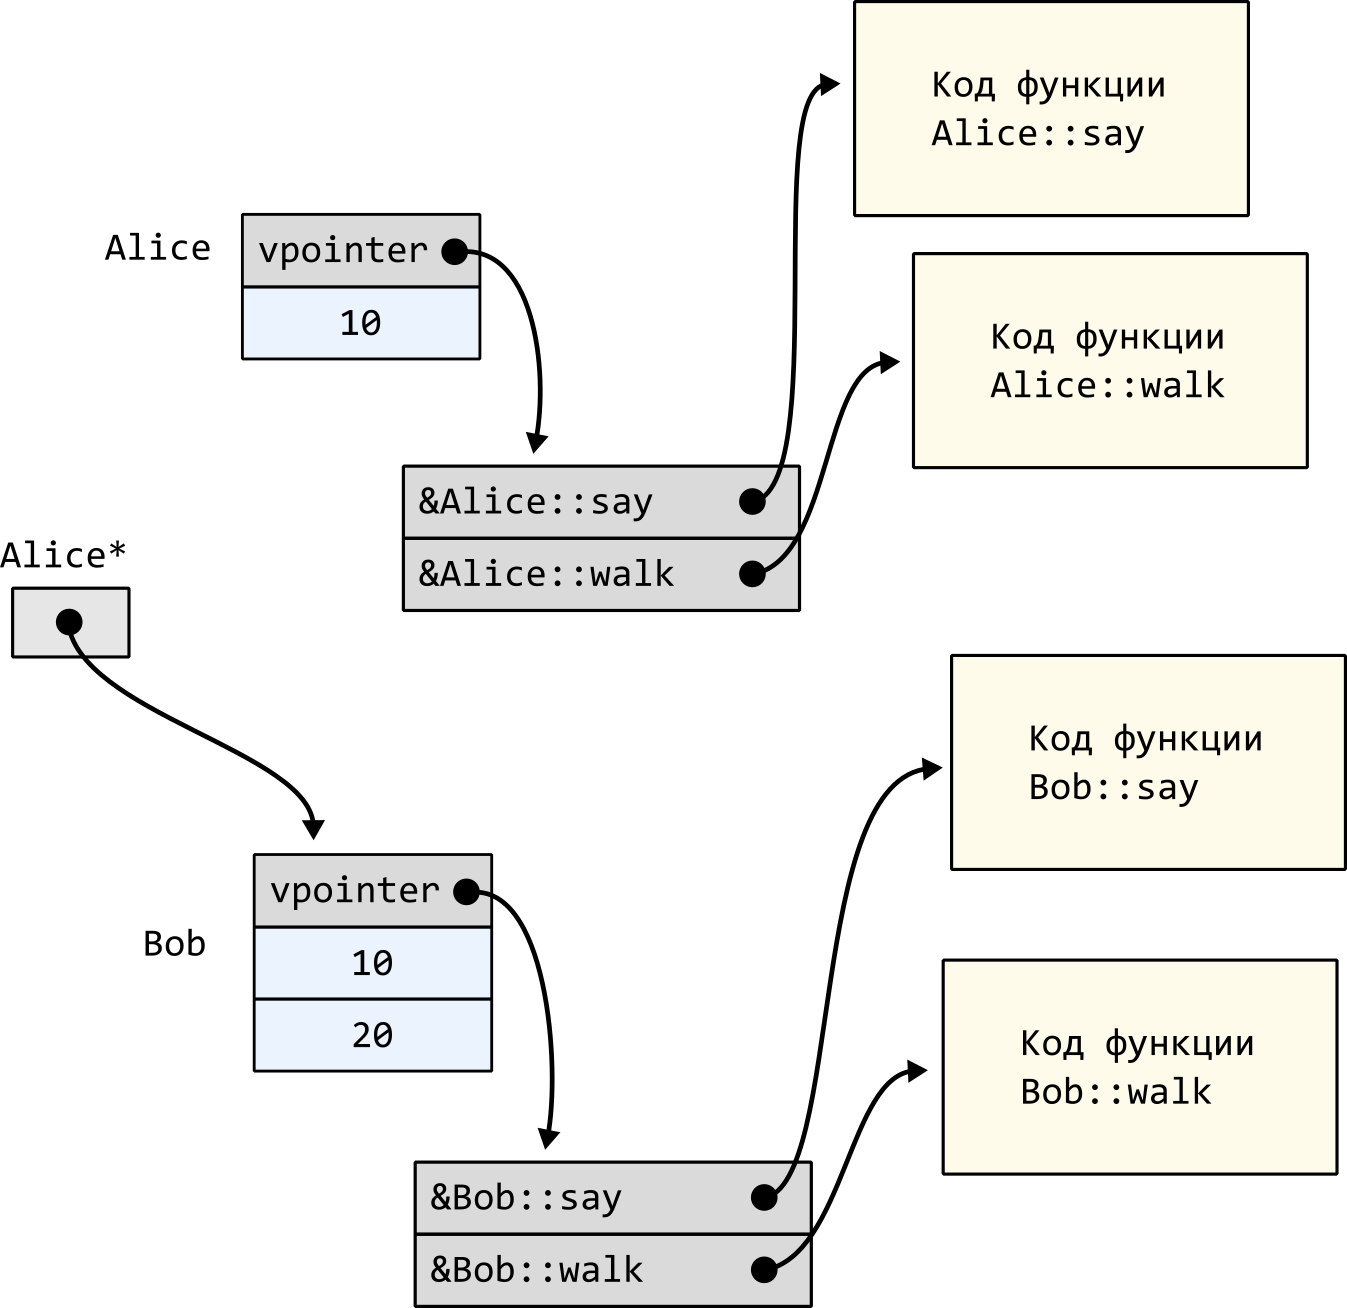
\includegraphics[scale=0.75]{../images/virtual_table_alice_bob.png}
\end{minipage}

\newpage


\section*{Абстрактные функции}
\subsection*{Чистые виртуальные функции}
\subsection*{Абстрактные классы и интерфейсы}
\subsection*{Контейнер указателей на базовый класс, хранящих адрес объектов производных классов}
\subsection*{pure virtual call и определение чистых виртуальных методов}


\section*{RTTI и \texttt{dynamic\_cast}}
\subsection*{Полиморфный тип}
\subsection*{\texttt{dynamic\_cast}}

\subsubsection*{\texttt{dynamic\_cast} от родителя к ребёнку}
\subsubsection*{\texttt{dynamic\_cast} в бок}

\subsection*{Оператор \texttt{typeid} и класс \texttt{std::type\_info}}


\end{document}
